% Chalmers title page
\begin{titlepage}

\AddToShipoutPicture{\backgroundpic{-4}{56.7}{fig/auxiliary/frontpage}}
\mbox{}
\vfill
\addtolength{\voffset}{2cm}

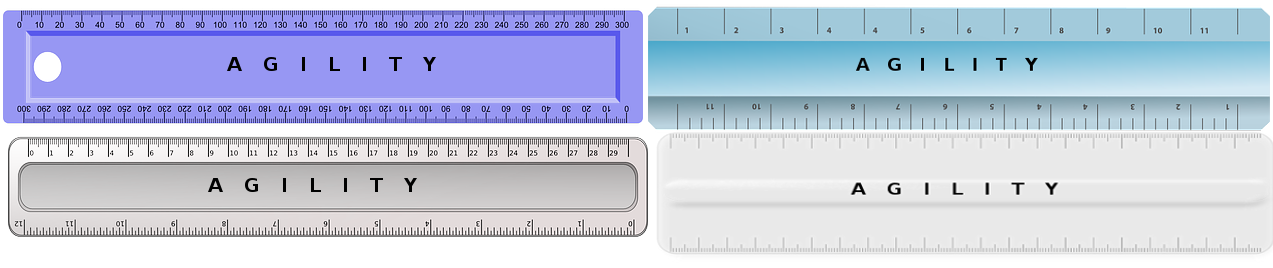
\includegraphics[scale=0.3]{fig/auxiliary/cover.png}
%http://pixabay.com/
	
\begin{flushleft}
	{\noindent {{\Huge Measuring Agility} \\[0.5cm] {\Large A Validity Study on Tools Measuring The Agility Level of Software Development Teams}} \\[0.5cm]
\emph{\Large Master of Science Thesis in Software Engineering} \\[.8cm]
	
	{\huge KONSTANTINOS CHRONIS}\\[.8cm]
	
	{\Large Chalmers University of Technology \\
    University of Gothenburg} \\
     Department of Computer Science and Engineering \\
     Göteborg, Sweden, June 2015
  } 
	
\end{flushleft}

\end{titlepage}
\ClearShipoutPicture
% End Chalmers title page

\pagestyle{empty}
\newpage
\clearpage
\mbox{}
\newpage
\clearpage
\thispagestyle{empty}

\begin{abstract}

\paragraph{Context:} 
In the past two decades, an increasing number of software development teams have been transitioning to agile. As a result, a need has emerged for measuring how agile these teams are. To satisfy this need, many researchers have created their own agile measurement tools. However, none of the tools managed to provide a substantial solution.

\paragraph{Objective:} 
Many tools have been created for measuring the agility of software development teams, thus creating a saturation in the field. Three tools were selected in order to validate whether they will yield similar results. These tools were the Perceptive Agile Measurement (PAM), the Team Agility Assessment (TAA) and the Objectives Principles Strategies (OPS).

\paragraph{Method:} 
The surveys for the three tools were given to the four software development teams of Company $A$. The survey questions were grouped into agile practices which were checked for correlation in order to establish convergent validity. In addition, we checked whether the questions identified to be the same among the tools would would be given the same replies by the respondents. Moreover, the coverage of agile practices was analysed by checking which tool covers more agile practices. The results were used to see whether the three tools yield similar results.

\paragraph{Results:} 
The correlations of the data gathered were very few and very low. As a result, convergent validity could not be established. In addition, the questions which were identified as the same among the tools did not have the same answers from the respondents. Moreover, \ac{OPS} was the tool covering the most agile practices. All the above provide evidence that the three tools do not yield similar results.

\paragraph{Conclusion:} 
We conclude that the area of measuring agility is still fertile and more work needs to be done. Based on the various agile practices covered by each tool, we believe that not all tools are applicable to every team but they should be selected on the basis of how a team has transitioned to agile. This study has set a milestone in the area and pinpoints the need for a better way to measure agility. 

\end{abstract}

\newpage
\clearpage
\mbox{}
\newpage
\clearpage
\thispagestyle{empty}
\section*{Acknowledgements}

I would like to thank
\begin{itemize}
	\item[] phd student Lucas Gren and Dr. Richard Torkar for all their help and support during the period I was conducting my Master's Thesis.
	\item[] Nick for allowing me to conduct this case study in Company $A$.
	\item[] the Swedish state for allowing me to study in one of its finest institutions.
	\item[] my parents for offering me the chance to study and become what I am. 
	\item[] more than anyone else, my girlfriend Tanja for constantly supporting me and believing in me even when I stopped believing in myself. \\[1cm]
\end{itemize}

\hfill Konstantinos Chronis, Gothenburg, Sweden \today

\newpage
\clearpage
\vspace*{\fill} 
\begin{quote} 
\centering 
{\Large \textit{Measure what is measurable and}} \\ 
{\Large \textit{make measurable what is not so.}} \\ 
\hspace{7cm} --- Galileo Galilei
\end{quote}
\vspace*{\fill}
\mbox{}

\newpage
\clearpage
\mbox{}
